\begin{frame} \frametitle{Big cells and small cells}
\vspace{2mm}
\begin{definition}
	A cell is \emph{big} if it has size at least $N^{\frac14}$. Otherwise it is \emph{small}.
\end{definition} \medskip

Small cells can be processed by brute force. For big cells we will need DCRs.
    \medskip

\begin{center}
	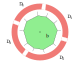
\includegraphics[width=5cm]{figs/consecDataStr}
\end{center}
\end{frame}

\def\mitem{\medskip\item}
\begin{frame} \frametitle{Description of data structure}
\begin{enumerate}
	\item Graph of VD in a form of adjacency list,
	\mitem {\it Dynamic nearest neighbor} structure for sites,
	\mitem Graph of big cells stored as adjacency list,
	\mitem For each big cell: \begin{itemize}
	     \mitem linked list of DCRs,
	     \mitem binary search tree of vertices in circular order.
	\end{itemize}
\end{enumerate}
\end{frame}

\begin{frame} \frametitle{Handling insertion}
\begin{block}{\vspace*{-3ex}}
	Initialize queue containing all the big cells and the cell of site closest to $s_N$. \\
	Look at cells one-by-one, on each step add to the queue unprocessed \\
	cells with changes. After all cells needing changes are in the queue, \\
	implement changes in them.
\end{block} \bigskip

\begin{itemize}
	\item Small cell: look at each paw to find neighboring cells needing changes, \\
	    add them to the queue.
	\mitem Big cell: ask DCRs to return Voronoi circles that enclose $s_N$, add
	    corresponding cells to the queue. When implementing changes \\
	    use graph of big cells to identify edges that have to be deleted. \\
	    Use BSTs to find the vertices that now belong to the cell of $s_N$.
\end{itemize} \vspace{7.5mm}
\end{frame}

\def\lrp#1{\left( #1 \right)}
\def\lrc#1{\left\lceil#1\right\rceil}

\begin{frame} \frametitle{Amortized expected runtime}
\def\otl{$\Ot(1)$ } \def\Ot{\tilde O}
\newcommand{\nof}{N^\frac{1}{4}}
\newcommand{\noh}{N^\frac{1}{2}}
\newcommand{\ntf}{N^\frac{3}{4}}

{\small $$
\Ot \lrp{
s\nof +
\sum_{i=1}^{|B|}  \lrp{ \lrc{\frac{|b_i|}{\nof }}+\ell_i}
+ \ntf + s\nof
}.
$$}

\begin{itemize}
	\item $s$ is $O(\noh)$ amortized\hfill\acite{incremental-vd},
	\mitem $\sum_{i=1}^{|B|} |b_i| \leq N$, $|B|\leq \ntf$,
	\mitem $\sum_{i=1}^{|B|} \ell_i \leq s \nof$.
\end{itemize} \bigskip

So this is simply {\large $$\Ot\ll\ntf\rr\quad\text{amortized.}$$}
\vspace{5mm}
\end{frame}